
\chapter{Installation and Usage}
\label{cha:installation-and-usage}

\section{Installation}

\begin{enumerate}
\item Download the zip archive and extract it to some folder. 
      (The binary build already includes a suitable Java Runtime Environment, so you do not need to install a JRE separately.)
    \item Start ASSIST by double clicking on ASSIST.exe (Windows only).
\end{enumerate}

\section{Usage}

ASSIST has been developed to support the following workflow:

\begin{enumerate}
\item Import or specify your hardware and software architecture in an \textbf{mdsl} file
\item Import or Specify your resource and safety requirements in the same \textbf{mdsl} file
\item Generate a set of valid deployments 
\item Sort these deployments according to customized metrics
\item Select an optimal deployment 
\item Export the selected deployment
\end{enumerate}

This can be achieved by:

\begin{enumerate}
\item Create a new project by clicking on \textsc{File} and \textsc{New}\\
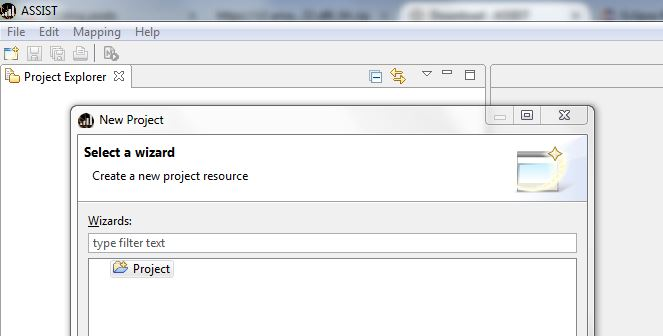
\includegraphics[width=0.8\textwidth]{gfx/install-new-project.jpg}\\
Please provide a suiteable name for your project and click on \textsc{Finish}.

\item Create a new mapping specification by clicking on \textsc{File} and \textsc{New}. Please select \textsc{Mapping Specification} in the following dialog.\\
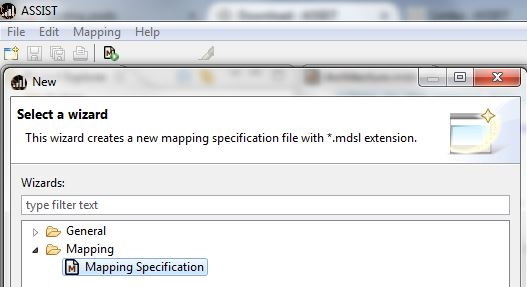
\includegraphics[width=0.8\textwidth]{gfx/install-new-mdsl-file.jpg}\\
Please provide a suiteable name for your deployment specification and click on \textsc{Finish}.

\item Mappings can be generated by clicking on \textsc{Mapping} and \textsc{Generate Mappings}\\
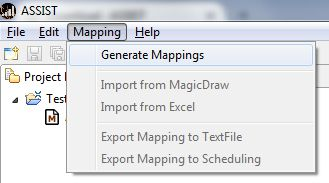
\includegraphics[width=0.5\textwidth]{gfx/install-generate-mappings.jpg}
\end{enumerate}

\section{Useful Shortcuts}

\begin{itemize}
\item \textbf{Ctrl-Shift-C} - Comment the current line or the currently selected lines
\item \textbf{Ctrl-Shift-F} - Format the current file (indention of sections, \dots)
\end{itemize}

%%% Local Variables:
%%% mode: latex
%%% TeX-master: "user-guide"
%%% End:
